\documentclass[review]{elsarticle}

\usepackage{lineno,hyperref}
\usepackage{subcaption}
\usepackage{siunitx}
\sisetup{group-separator = {,}}
\usepackage{booktabs}
\usepackage{graphicx}
\usepackage{adjustbox}
\usepackage{appendix}
\usepackage{amsmath} 
\usepackage{scrextend}
\usepackage[hang,flushmargin]{footmisc} 
\usepackage{xcolor}
\usepackage{float}
\usepackage{array,multirow}
\usepackage{hyperref}
\usepackage{setspace}
\usepackage{stmaryrd}
\usepackage{enumitem}
\usepackage{rotating}
\usepackage{adjustbox}
\usepackage{array}
\usepackage{booktabs}
\usepackage{xcolor,colortbl}
\usepackage{amsmath} 
\usepackage{amsfonts} 
\usepackage{amssymb}
\usepackage{makecell}
\usepackage{amsmath}
\usepackage{nicefrac}
\usepackage{todonotes}
\usepackage{multirow}
\modulolinenumbers[1]
\usepackage{lineno}
\usepackage{tikz}
\usepackage{cleveref}
\usepackage{accents} 
\usepackage{arydshln}
\usepackage[T1]{fontenc}
\linenumbers

% \usepackage[final]{changes}
\usepackage[markup=underlined]{changes}

\usepackage[ruled,vlined,linesnumbered,lined,boxed,commentsnumbered]{algorithm2e}
\newcommand\mycommfont[1]{\footnotesize\ttfamily\textcolor{blue}{#1}}
\SetCommentSty{mycommfont}
\newcommand{\BREAK}{\STATE \algorithmicbreak}
\modulolinenumbers[1]
\setlength{\parindent}{0em}
\journal{Energy}
\bibliographystyle{elsarticle-num}

\begin{document}
\begin{frontmatter}

\title{Shrinking together and pulling apart: the Austrian gas grid by 2040 under declining natural gas demand and increasing domestic renewable gas generation}
\author[1,2]{Sebastian Zwickl-Bernhard\corref{cor1}}
\ead{zwickl@eeg.tuwien.ac.at}
\author[3]{Aria Rodgarkia-Dara}
\author[3]{Christoph Gatzen}
\author[1]{Marcus Otti}
\author[1]{Antonia Golab}
\author[1,2]{Hans Auer}
\cortext[cor1]{Corresponding author}
\address[1]{Energy Economics Group (EEG), Technische Universität Wien, Gusshausstrasse 25-29/E370-3, 1040 Wien, Austria}
\address[2]{Industrial Economics and Technology Management, Norwegian University of Science and Technology, Gløshaugen, Alfred Getz vei 3, Trondheim, 7491, Norway}
\address[3]{Frontier Economics Limited, 71 High Holborn, London WC1V 6DA, United Kingdom}

\begin{abstract}
\end{abstract}

\begin{keyword}

\end{keyword}
\end{frontmatter}
%
%\newpage
%\section*{Nomenclature}
%\begin{center}
%	\renewcommand{\arraystretch}{1.0}
%	\centering
%	\small
%	\begin{tabular}{lm{7.75cm}r}
%		Type & Description & Unit\\
%		\hline
%		Set and index & & \\
%		\hline
%		{$p \in \mathcal{P}=\{1,\ldots,P\}$} & Pipeline for gas transport, index by $p$\\
%		{$n \in \mathcal{N}=\{1,\ldots,N\}$} & Node of the gas network, index by $n$\\
%		{$l \in \mathcal{L}=\{1,\ldots,L\}$} & Gas network level (e.g., high-pressure), index by $l$\\
%		{$y \in \mathcal{Y}=\{1,\ldots,Y\}$} & Years, index by $y$\\
%		{$m \in \mathcal{M}=\{1,\ldots,M\}$} & Months, index by $m$\\
%		\hline
%		\multicolumn{2}{l}{Primal Decision Variables (Selection)}\\
%		\hline
%		{$Capex$} & Capital expenditures & \SI{}{EUR}\\
%		{$Opex$} & Operational expenditures & \SI{}{EUR}\\
%		{$Rev$} & Revenues generated by gas supply & \SI{}{EUR}\\
%		{$\gamma_{p,l,y}$} & Capacity of pipeline $p$ at $l$ in $y$& \SI{}{MW}, \SI{}{GW}\\
%		{$q^{dem}_{n,l,y,m}$} & Gas demand supplied at $n$ and $l$ in $y$ and $m$ & \SI{}{MWh}, \SI{}{GWh}\\
%		{$q_{p,l,y,m}$} & Quantity of gas transported at $p$ and $l$ in $y$ and $m$& \SI{}{MW}, \SI{}{GW}\\
%		{$\Pi_{p,l,y}$} & Book value of pipeline $p$ at $l$ in $y$ & \SI{}{EUR}\\
%		\hline
%		\multicolumn{2}{l}{Dual Decision Variables}\\
%		\hline
%		{$\lambda^{CO}_{n,l,y,m}$} & Cost-optimal shadow price of gas supply without ensured supply at $n$ and $l$ in $y$ and $m$ & \SI{}{EUR \per MWh}\\
%		{$\lambda^{ES}_{n,l,y,m}$} & Cost-optimal shadow price of gas supply with ensured supply at $n$ and $l$ in $y$ and $m$ & \SI{}{EUR \per MWh}\\
%		\hline
%		\multicolumn{2}{l}{Parameters (Selection)}\\
%		\hline
%		{$\gamma^{pre}_{p,l,y}$} & Preexisting capacity of pipeline $p$ at $l$ in $y$ & \SI{}{MW}, \SI{}{GW}\\
%		{$d^{max}_{n,l,y,m}$} & Maximum gas demand at $n$ and $l$ in $y$ and $m$ & \SI{}{MWh}, \SI{}{GWh}\\
%		{$q^{fed}_{n,l,y,m}$} & Quantity of gas fed in at $n$ and $l$ in $y$ and $m$ & \SI{}{MW}, \SI{}{GW}\\
%		{$c^{inv}_{l}$} & Specific refurbishment investment costs at $l$  & \SI{}{EUR \per MW \per km}\\
%		{$\Pi^{pre}_{p,l,y}$} & Book value of preexisting pipeline $p$ at $n$ in $y$& \SI{}{EUR}\\
%		{$y^{inv}_{p,l}$} & Year of refurbishment/decommissioning per $p$ and $l$ & \SI{1}{}\\
%		{$\omega$} & Weighted average cost of capital & \SI{}{\%}\\
%		{$i$} & Interest rate (for calculating the net present value) & \SI{}{\%}\\
%		\hline
%	\end{tabular}
%\end{center}
\newpage

\section{Introduction}
Adherence to the remaining CO\textsubscript{2} budget of the Paris Agreement requires rapid defossilization of the energy system \cite{rockstrom2017roadmap}. In Europe, the \textit{Fit for 55} package \cite{european_commission_european_2019} and the \textit{EU Green Deal} \cite{greendeal} define the mid- and long-term goals for a transition to a sustainable energy supply until the middle of the century. These goals include a reduction of CO\textsubscript{2} emissions by 55\% compared to those in 1990 by 2030 and climate neutrality in 2050. In light of this, the question of the concrete design of measures to achieve these goals arises \cite{hainsch2022energy}. Numerous scientific works have already been dedicated to the analysis of sustainable alternatives for the provision of energy service needs, which currently rely on fossil fuels. Abas et al. \cite{abas2015review} provide a comprehensive review of fossil fuels as a primary energy source in the energy supply chain and future energy technologies. Corresponding studies, \added[]{(e.g., \cite{hainsch2022energy} and \cite{abas2015review}),} \replaced[]{often}{frequently} focus primarily on the renewable energy technology portfolio that provides energy service needs in the future. We essentially use these as the starting point of our analysis here, investigating implications of expected declining coverage of energy services by natural gas, a fossil fuel, on its transmission and distribution network infrastructure.\vspace{0.35cm}

Natural gas is undeniably one of the pillars of existing energy systems, but it is being fundamentally challenged by the already established and ongoing decarbonization of energy systems. Furthermore, as part of the sustainable transition, natural gas and its role are expected to undergo significant transformation.\footnote{McGlade and Ekins \cite{mcglade2015geographical} state that half of natural gas reserves should remain unused from 2010 to 2050 in order to meet at least the less ambitious 2.0°C climate target from the Paris Agreement.} However, presently, it is not clear which exact trajectory natural gas will take until 2050 \cite{safari2019natural}.\footnote{Exemplarily, Kumar et al. \cite{kumar2011current} see natural gas as an important bridging fuel to a sustainable energy system, in some cases even after 2050. By contrast, Stephenson et al. \cite{stephenson2012greenwashing} propose to abandon the transition fuel characterization of natural gas. D{\'\i}az et al. \cite{diaz2017we} follow this point of view since they find for the electricity sector that natural gas delivers little to no cost savings as a bridging fuel in a system that switches to wind and solar.} Two focal reasons/subjects are (i) various energy sectors currently use natural gas in the provision of energy services (e.g., generation of process heat or as a base material for industrial consumers, centralized generation of electricity and district heating, and decentralized supply of space heating and hot water demands), and it is not clear if and when exactly sustainable alternatives will be economically available, implemented, and realized in sufficient quantities \cite{mohseni2013competitiveness, gorre2019production}. (ii) Synthetic gases (including hydrogen) are seen as a promising alternative or supplement to natural gas usage, as they could be fed into existing transmission and distribution gas network infrastructure, although there are valid uncertainties regarding its amount of technical as well as economic potentials \cite{lux2020supply, blanco2018potential}. Because of that, the question is not only which energy sectors and energy services remain to use the limited quantities of natural (following the trend of defossilization) and synthetic (because of limited potentials gas) but also what gas network infrastructure will continue to be needed for their transport and distribution.\vspace{0.35cm}

The goal of this paper is to contribute to scientific research on its future development and trajectory of gas network infrastructure with the expectation of decreasing natural gas demands and increasing the integration of green gases, such as synthetic gas and hydrogen. The emphasis is on gas network infrastructure, which ensures that various energy service needs (e.g., residential building heat, and industrial process heat) are met. This raises the question of which gas network infrastructure is required to meet non-substitutable natural gas demands when considering possible stand-alone natural gas supply options (e.g., delivery of liquefied natural gas by truck) \added{in order to avoid significant economic loss and stranded assets in the future. To meet demand, the network can transport either imported gas volumes or locally produced green gases such as biomethane.} Nonetheless, even if stand-alone solutions are viable alternatives in some cases, arbitrariness regarding the trajectory decisions of gas networks must be avoided, as they are not only assigned to critical infrastructure but also regulated and subject to long-term energy planning (lock-in effect).\vspace{0.35cm} 

The primary objective of this work is to investigate the cost-effective trajectory of gas network infrastructure from a systemic viewpoint under a long-term planning horizon. Given necessary refurbishment investments in existing gas network infrastructure and pipelines due to their technical lifetimes, the main research question is which decommissioning and refurbishment investment decisions result in a cost-effective gas network infrastructure by 2050. Equally important in the analysis is the network operator's trade-off decision regarding whether available gas demands within the network area are supplied or not, as decommissioning of existing gas pipelines can be cost-effective but results in unsupplied gas demands. Consequently, three different model runs are performed, allowing a thorough comparison of various handling options in terms of gas demands not met by the network infrastructure.\footnote{Grid operator usually is a regulated entity. Thus, finally, it is a regulatory question/decision which cannot be taken by the grid operator alone (regulator).} Accordingly, analysis relies heavily on the shadow prices of gas supply at the local level within the network's nodes. \added{At present, existing studies on gas network infrastructure are insufficient, and the corresponding literature has not yet conducted a comprehensive comparison of different sub-policy implications for handling future gas demands by a quantitative analysis.}\vspace{0.35cm}

The method used is the development of a linear optimization model. Thereby, the objective function is to minimize the network operator's net present value over time. Particularly, the optimal solution of the model includes the decommissioning and refurbishment investment decision of parts of the network and single pipelines. This includes deciding whether or not to supply available gas demand. The dual variables of the local gas balance constraints allow us to assess the techno-economic range of supply alternatives for each node in the network.\vspace{0.35cm}

The numerical example examined is a small portion of the existing Austrian gas network infrastructure in the NUTS2 region Vorarlberg, Austria. This area is distinguished by a wide range of energy service requirements that are met by natural gas (e.g., residential, and industry). Furthermore, the gas network infrastructure includes not only high- and mid-pressure network connections but also cross-border connections to neighboring countries Germany and Lichtenstein (i.e., transmission network level). There is also the possibility of producing green gas and injecting it into the existing gas network infrastructure.\vspace{0.35cm}

The paper is organized as follows. Section \ref{stateoftheart} provides an overview of the current state-of-the-art in scientific literature and outlines the novelties of this work beyond existing research. Section \ref{methodology} presents the materials and methods developed in this work, including, the model's mathematical formulation and description of different model runs. Section \ref{results} presents the results of this work encompassing different handlings of gas demands within the network. Section \ref{conclusions} synthesizes and discusses the results, concludes the work, and gives an outlook for future research.  
\newpage
\section{State-of-the-art and progress beyond}\label{stateoftheart}
This section discusses relevant scientific literature in the field of this work. It is divided into three parts. First, Section \ref{import} deals with the global and cross-country dimension of natural and renewable gas trade. It focuses on the impact of the decarbonization on gas markets and discusses also intra-country gas supply with a high spatial granularity of a grid representation. Then, Section \ref{approaches} examines different approaches of modeling gas grids. Section \ref{tariffs} elaborates on the regulation of gas grids and especially on gas grid charges. Finally, Section \ref{novelties} highlights the novelties of this work. Due to the complexity of the topic and the associated magnitude of possible relevant literature, what is not part of the literature review is briefly discussed. \textcolor{red}{Hier beschreiben was nicht part ist.} % Literature that examines the entire energy system across sectors is not considered. Instead, those studies are considered that focus primarily on the gas sector, as is the case in the present work. Literature that deals with the gas sector but does not consider the network is also excluded.  

\subsection{Decarbonized gas markets and cross-country trade}\label{import}

In 2021, the European Commission has published a proposal for a framework of renewable and natural gases and for hydrogen \cite{regulation_renewable_gases}. The aim is to support renewable and low carbon gases (i.e., biogas, biomethane, renewable and low carbon hydrogen as well as synthetic methane) in Europe and to reach a share of two-third of gaseous fuels in 2050 energy mix. Further details on the definition of renewable and low carbon gases can be found in \cite{briefing_renewable_gases}. The remaining one-third of gaseous fuels in 2050 is expected to be still fossil natural gas, but in combination with carbon capture, storage and utilization. Today, renewable and low carbon gases have only a minor contribution to Europe's energy mix. Bertasini et al. \cite{bertasini2023decarbonization} give a critical overview of the contribution of renewable gases to the decarbonization of the European energy system and grids. Kolb et al. \cite{kolb2021scenarios} focus in their work on the integration of renewable gases into gas markets. In addition, the latter study provides also a comprehensive literature review on the topic of renewable gases. Lochner \cite{lochner2011identification} elaborates on the European gas market and the identification of congestions in the gas transmission grid. Gorre et al. \cite{gorre2019production} deal exhaustively with future renewable gas generation costs.\vspace{0.3cm}

A key role in the transition to renewable and low carbon gas markets has the existing gas infrastructure. On the hand, the repurposing of existing pipelines especially at the transmission grid level allow to build up a hydrogen grid, as proposed in the so-called "Hydrogen Backbone" \cite{hydrogen_backbone}. In this context, also the recently extended terminal capacities for liquified natural gas (LNG) are worth to be mentioned. In the short-term, LNG terminals are used to support Russian natural gas import substitution by fossil LNG imports from exporter countries, such as the United States and Quatar \cite{brauers2021liquefied}. But in the mid-term, these terminals can be used to import renewable and low carbon gases, supporting the European gas market \cite{al2022emerging}. On the other hand, the area-wide existing pipelines of the distribution grid levels (high-, mid-, and low-pressure pipelines) allow the injection of distributed renewable and low carbon gas generation \cite{cucchiella2018profitability}. Sulewski \cite{sulewski2023development} explore the biomethane market in Europe. Schlund and Schönfisch \cite{schlund2021analysing} analyze the impact of renewable quota on the European natural gas markets. Paturska et al. \cite{paturska2015economic} provide an economic assessment of biomethane supply system based on the natural gas grid. Khatiwada \cite{khatiwada2022decarbonization} elaborate on barriers of the decarbonization of natural gas systems. Stürmer \cite{sturmer2020greening} examines in detail on the potentials of renewable gas injection into existing gas grids. 

\subsection{Gas grid modeling approach (top-down and bottom-up)}\label{approaches}
The following literature review focuses on the modeling of natural gas transport by grids and pipelines. There are other ways of transporting natural gas. The interested reader is referred to Thomas and Dawe \cite{thomas2003review} for a comprehensive review of the options for transporting natural gas. In general, the literature on gas grid modeling approaches can be divided based on two key dimensions: (i) modeling perspective (e.g., techno-economic) and (ii) spatial scale. These dimensions, along with others such as the sectoral dimension (whether or not hydrogen is accounted for in detail), determine the level of consideration given to various factors such as flow conditions of natural gas, pressure levels and drops in transport pipelines, and the operational energy and costs associated with compressors.\vspace{0.3cm}

A review on optimization of natural gas transportation systems is given by R{\'\i}os-Mercado and Borraz-S{\'a}nchez \cite{rios2015optimization}. It encompasses both transmission and distribution grids. Pfetsch et al. \cite{pfetsch2015validation} elaborate in detail on the operation of gas transmission grids. Pambour et al. \cite{pambour2016integrated} propose an integrated transient model approach for simulating the operation of transmission grids. The transient process in transmission grids is further examined by Liu \cite{liu2011coordinated}. Riepin et al. \cite{riepin2022adaptive} develop in their study an adaptive robust optimzation model for transmission grid expansion planning. Chiang and Zavala \cite{chiang2016large} investigate the interconnection between gas and power transmission grids. O'Donoghue et al. \cite{o1997development} examine transmission pipelines' resistance to high-pressure levels. Liu et al. \cite{liu2009security} study aspects of supply security in detail.\vspace{0.3cm}

With regard to the distribution grid level, Herr{\'a}n-Gonz{\'a}lez et al. \cite{herran2009modeling} provide a comprehensive review on the modeling and simulation of gas grids. Barati et al. \cite{barati2014multi} propose an integrated framework for grid expansion planning.  Giehl et al. \cite{giehl2023assessment} examine the impact of the decarbonization on gas distribution grids. Zwickl-Bernhard and Auer \cite{zwickl2022demystifying} present alternative supply options to natural gas distribution grids. Keogh et al. \cite{keogh2022gas} review technical and modeling studies of renewable gas generation and injection into the distribution grid. The same authors present also a techno-economic case study for renewable gas injection into the distribution grid in \cite{keogh2022gas}. Abeysekera et al. \cite{abeysekera2016steady} analyze the injection of renewable gas in low-pressure gas grids from a technical perspective in detail. Mertins et al. \cite{mertins2023competition} examine the competition between renewable gas and hydrogen injection into distribution grids. Repurposing of natural gas pipelines for hydrogen transport is assessed by Cerniauskas et al. \cite{cerniauskas2020options}. An overview of the modeling of hydrogen grids is given by Reuß et al. \cite{reuss2019modeling}.\vspace{0.3cm}

Finally, the modeling contributions of the open-source community subject of gas grids are discussed. In principle, open-source approaches are becoming increasingly important in energy system analysis \cite{hulk2018transparency}. This trend is also continuing in the area of gas grids. For instance, Schmidt et al. \cite{schmidt2017gaslib} provide a set of publicly available gas grid instances that can be used by researchers in the field of gas transport. Pluta et al. \cite{pluta2022scigrid_gas} present an approach for developing an open-source model of the gas transport grid in Europe. Nevertheless, data on natural gas grids in particular are rarely made publicly available. There are isolated exceptions, e.g. for the transmission grid (see \cite{entsog} for open-source data on the European transmission gas grid) or for the Belgian gas grid in \cite{de2000gas}. However, there is often an information advantage for those who have this information (e.g., gas grid operators) to scientific researchers, particularly with analyses at the distribution grid level. 

\subsection{Decarbonized gas grid regulation}\label{tariffs}
% Sehr wenig Literatur dazu wie die Regulierung bzw. Endkundentarifgestaltung in dekarbonisierten Gasnetzen aussehen kann. 
% Deutlich mehr Literatur besteht im Zusammenhang mit Stromnetzen auf dem Weg Richtung decarbonized.
% Hier 2-3 Literaturstellen zu Power Grid Tariff Renewables erwähnen.
% sehr wichtig weil auch tariff regulation long-term estimates until 2050; renewable and low-carbon gases
% dann hier diesen französischen bericht zitieren.
% Bouacida et al. \cite{bouacida2022impacts}: Impacts of greenhouse gas neutrality strategies on gas infrastructure and costs: implications from case studies based on French and German GHG-neutral scenarios
% dann das eigene paper zitieren wo von sozialisierung der kosten gesprochen wird. 






\subsection{Novelties}\label{novelties}

- techno-economic open-source modeling approach of gas transmission and distribution grids with focus on the replacement and decommissioning investment decision up to 2050

- langristige abschätzung von netzkosten tariffen, erstmaliger kostenvergleich/abschätzung was elektrifizierung des energiesystems für das gasnetz konkret bedeutet

- application to the Austrian gas grid das besonders  spannend ist weil es ein hohes potential für biomethane integration hat

- open-source approach





\newpage
 \section{Method}\label{methodology}
This section describes the methodology of the paper. First, in Section \ref{model}, the optimization model used is explained in detail. The focus is thereby on the mathematical formulation. However, where meaningful, qualitative explanations are added to give the reader a more complete understanding of the model. These qualitative explanations are used in particular to describe the main decision made by the model between maintaining operation, decommissioning or making replacement investment in existing gas grid pipelines. In Section \ref{gas_grid_austria}, the gas grid in Austria, which serves as the case study in this paper is presented. Then, in Section \ref{scenarios}, the four different scenarios are shown. Finally, Section \ref{data} provides information on the data used, while Section \ref{limitations} takes a critical look at the method and discusses some limitations and their impact on the results.
 
 \subsection{Optimization model}\label{model}
 
 
 \begin{figure}[h]
 	\centering
 	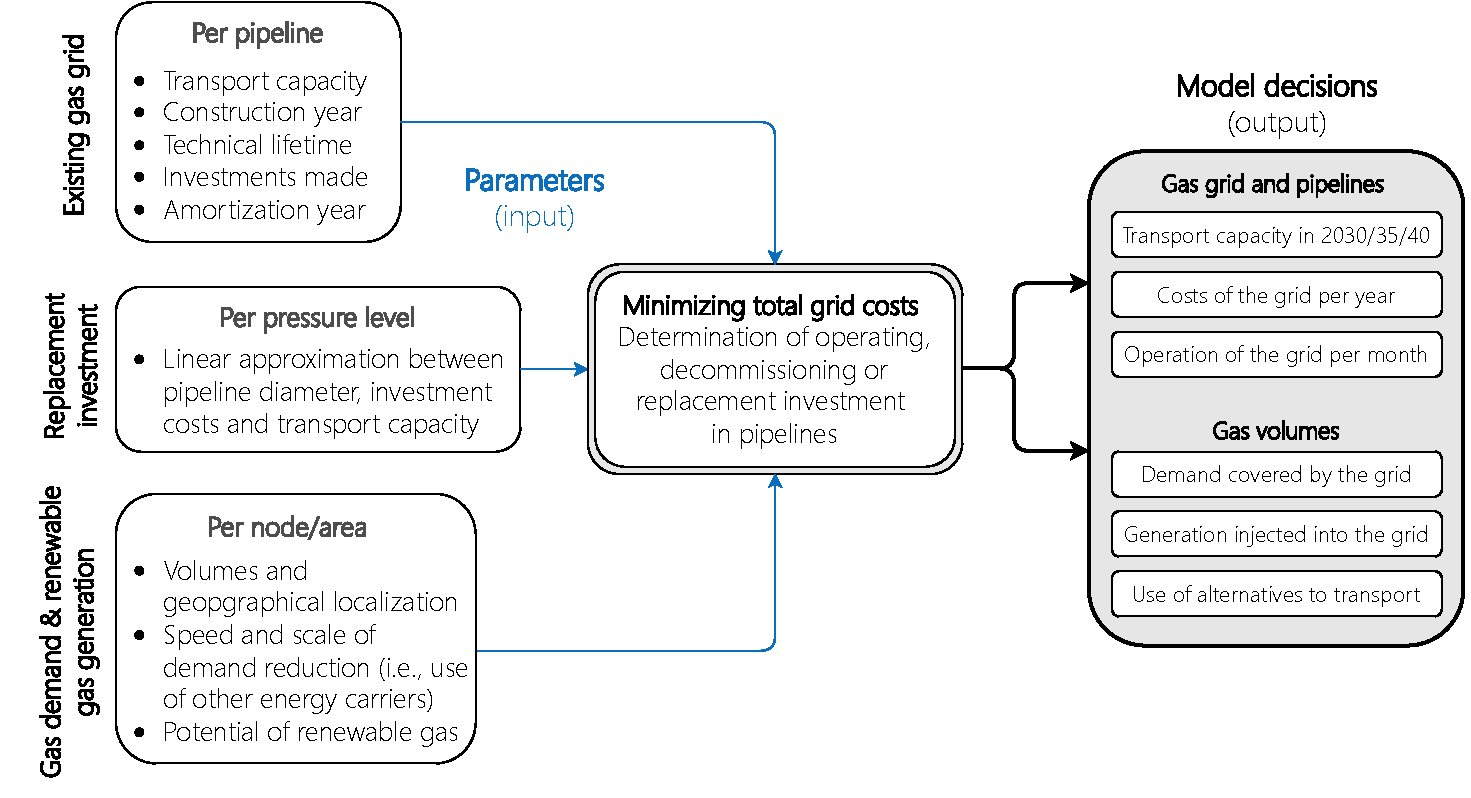
\includegraphics[width=1\linewidth]{figures/method/overview.pdf}
 	\caption{}
 	\label{}
 \end{figure}
 
 \subsubsection{Overview}
 
 % graphen basiertes model
 % schaut nur auf den energieträger gas
 % gas balance constraint per node
 
 % übersichtsgrafik was sind die inputs, was die outputs
 
 \subsubsection{Objective to minimize total grid costs}
 
 \subsubsection{Operation, decommissioning or replacement investment in pipelines}
 
 \subsubsection{Further constraints}
 
 % The set of supplied and discharged flows, together with additional specifications on the supplied and discharged gas pressures and the chemical compositions of the supplied gas, is called a nomination.
 
 % In stationary models, it is typically assumed that the sum  of supplied flows equals the sum of the discharged flows, that is, the nominations have to be balanced.

 

 
 
 

 \subsection{Existing gas grid in Austria}\label{gas_grid_austria}
 
 \subsection{Scenarios}\label{scenarios}
 
 \subsection{Data}\label{data}
 
 \subsection{Limitations}\label{limitations}
 % Schreiben dass es nicht zwingen notwendig sein muss holistisch darauf zu blicken
 
 % Druckniveaus
 % Umhängen von Verbrauch

 
 
 
 
 % 1) Optimierungsmodell
 	% 1.1 Übersicht über das Modell
 	% 1.2 Wesentlichen Funktionalitäten
 % 2) Szenarien
 	% Übersicht über die Szenarien 
 	% worin unterscheiden sich die Szenarien
 	% Detaillierte Beschreibung der Szenarien
% 3) Test-bed

 
 
 
 % vor dem ende der technischen lebensdauer
 % zum zeitpunkt des ablaufs der technischen lebensdauer
 
% This section explains the proposed methodology. First, Section \ref{Met:Intro} introduces the model. Then, Section \ref{Met:Equations} presents the mathematical formulation in detail. Section \ref{runs} explains the different model runs and defined scenarios. Section \ref{testbed} provides the test bed description and shows the gas networks in Vorarlberg, Austria, in detail, and Section \ref{label:inputs} presents the input data. Section \ref{label:limitation} discusses the limitations of the model. Finally, Section \ref{environment} deals with the open-source programming environment and the computation time of the model. 
% 
% \subsection{Introduction of the model}\label{Met:Intro}
% Figure \ref{fig:methodology} provides an overview of the method, including the interrelationships between the inputs (left), the \replaced{model}{modeling framework} (middle), and the outputs (right). Generally, the inputs (and thus parameters) can be divided into three different categories, namely, technical parameters (e.g., existing pipeline capacity per network/pressure level and the year of construction), economic parameters (e.g., refurbishment investment costs per pipeline), and further empirical data needs (e.g., gas demand and supply at the local community level and seasonal gas storage capacities). The \replaced[]{model}{modeling framework (CANCEL)} is developed as a linear program and is based on graph theory. It emphasizes the high spatial resolution in modeling. Particularly, a single node in the gas network graph corresponds to a community and covers an area of approximately \SI{40}{km^2} on average. The temporal resolution and thus investment planning horizon are until 2050, whereas an individual year is monthly resolved. \replaced[]{The model outputs include the optimal investment and dispatch decisions.}{Since the modeling framework is an investment and dispatch model, the outputs can also be divided into these catergories.} The outputs related to the investment decision are particularly the decommissioning and refurbishment investment decision per pipeline and gas network level. Additionally, the outputs encompass the dispatch of the gas networks on a monthly resolution. This includes the utilization of pipelines and particularly the gas demand and gas demand not supplied per community. 
% 
%  \begin{figure}[h]
% 	\centering
% 	\includegraphics[width=1\linewidth]{figures/flowchart.pdf}
% 	\caption{Overview of the method}
% 	\label{fig:methodology}
% \end{figure}
% 
% \subsection{Mathematical formulation}\label{Met:Equations}
% This section is dedicated to providing a detailed mathematical formulation of the \replaced[]{model}{modeling framework}. We start with the objective function and have deliberately chosen the further order of equations so that the following equation builds on the previous one as far as possible. \added[]{In addition to the detailed description of the equations below, Table} \ref{tab:brief} in \ref{app_overview} \added[]{summarizes the main equations of the model with a qualitative explanation.}\vspace{0.35cm}
% 
% Equation \ref{objective} shows the objective function of the model where $Capex$ is the net present value of the capital expenditures, $Opex$ of the operational expenditures, $Rev$ of the revenues from the supply of gas demands, and $Purch$ of purchasing gas. $Capex$ and $Opex$ represent the decommissioning and investment decision, whereas $Rev$ and $Purch$ the dispatch of the gas networks.  
% \begin{align}\label{objective}
%  	\underset{x}{\mathrm{min~}} Capex + Opex - Rev + Purch
%  \end{align}
%Additionally, $x$ represents the decision variables of the model. \added{All costs and prices are nominal.} Equation \ref{discount} shows the calculation of the discount factor per year $y$ ($\alpha_y$), where $i$ is the interest rate and $y_0$ is the reference year. 
%\begin{align}\label{discount}
%	\alpha_y = \frac{1}{(1+i)^{y-y_0}}
% \end{align}
%Building upon, $Capex$ is calculated as shown in Equation \ref{eq:capex} where $\omega$ is the weighted average cost of capital and $\Pi_y$ is the book value of the pipelines in $y$.
%\begin{align}\label{eq:capex}
%	Capex = \sum_{y}^{y_{end}-1} \alpha_y \cdot \omega \cdot \Pi_y + \underbrace{\alpha_{y_{end}} \cdot \Pi_{y_{end}}}_{\text{early depreciation}}	
%\end{align}
%Similarly, $Opex$ is calculated as shown in Equation \ref{eq:opex} where $\lambda_y$ is the fixed (operating) costs of the pipelines in $y$. 
%\begin{align}\label{eq:opex}
%	Opex = \sum_{y} \alpha_y \cdot \lambda_y
%\end{align}
%Equation \ref{eq:lambda} shows the calculation of the $\lambda_y$ where $c^{fix}_{l}$ is the specific fixed (operating) costs per $l$ and $\gamma_{l, y}$ is the installed pipeline capacity per $l$ in $y$.
%\begin{align}\label{eq:lambda}
%	\lambda_y = \sum_{l} c^{fix}_{l} \cdot \gamma_{l, y}
%\end{align}
%Equation \ref{eq:gamma} shows the calculation of $\gamma_{l, y}$ where $\gamma_{p,l,y}$ is the installed pipeline capacity at $p$ and $l$ in $y$ and $P_{l}$ the subset of all pipelines at $l$. \added[]{$\Lambda_{p}$ is a scaling factor. It is needed because the parameter $c^{fix}_{l}$ is defined for a representative pipeline length for each pressure level. These representative pipeline lengths are 50km and 25km for the high-pressure and mid-pressure network levels respectively. For example, if a pipeline $p$ at the high-pressure network level has a length of 50km, then the scaling factor $\Lambda_{p}$ is equal to 1. Note that $\Lambda_{p}$ is known a priori (because the length of pipelines are known) and is a parameter of the model.}
%\begin{align}\label{eq:gamma}
%	\gamma_{l, y} = \sum_{p \in P_{l}} \Lambda_{p} \cdot \gamma_{l, y, p}
%\end{align}
%Equation \ref{eq:total_capacity} defines the capacity of a pipeline $p$ at $l$ in $y$ where $\gamma^{pre}_{p,l,y}$ is the preexisting capacity and $\gamma^{ref}_{p,l,y}$ is the refurbished capacity of $p$ at $l$ in $y$. 
%\begin{align}\label{eq:total_capacity}
%	\gamma_{p,l, y} = \gamma^{pre}_{p,l,y} + \gamma^{ref}_{p,l,y}
%\end{align}
%Similarly, Equation \ref{eq:total_book_value} defines the book value of a pipeline $p$ at $l$ in $y$, where $\Pi^{pre}_{p,l,y}$ is the book value of the preexisting pipeline (capacity), $\Pi^{ref}_{p,l,y}$ of the refurbished capacity of $p$ at $l$ in $y$, and $f^{ref}_{p,l}$ the discount factor at $p$ and $l$.
%\begin{align}\label{eq:total_book_value}
%	\Pi_{p,l,y} = \Pi^{pre}_{p,l,y} + f^{ref}_{p,l} \cdot \Pi^{ref}_{p,l,y^{inv}_{p,l}}
%\end{align}
%Equation \ref{eq:tbv} sums the book values of all pipelines and network levels to obtain the total book value per $y$ ($\Pi_y$).
%\begin{align}\label{eq:tbv}
%	\Pi_{y} = \sum_{p} \sum_{l} \Pi_{p,l,y}
%\end{align}
%The following equation defines the refurbished installed capacity per $p$ at $l$ in $y$ resulting from the refurbishment (or decommissioning) decision in the year of the decision ($y^{inv}_{p,l}$).
%\begin{align}\label{9}
%	\gamma^{ref}_{p,l,y} = \begin{cases}
%		0 & \quad:\forall y~|~y<y^{inv}_{p,l}\\
%		\gamma^{ref}_{p,l,y-1} & \quad:\forall y~|~y>y^{inv}_{p,l}
%	\end{cases}
%\end{align}
%Equation \ref{eq:bvalue_ref} calculates the book value of the refurbishment investment at $p$ and $l$ in $y^{inv}_{p,l}$.
%\begin{align}\label{eq:bvalue_ref}
%	\Pi^{ref}_{p,l,y^{inv}_{p,l}} = c^{inv}_{l} \cdot \gamma^{ref}_{p,l,y^{inv}_{p,l}}
%\end{align}
%Equations \ref{exp} and \ref{imp} define the total gas export and import from $n$ at $l$ in $y$ and $m$ where $q_{p,l,y,m}$ is the amount of gas transported by $p$ at $l$ in $y$ and $m$. Additionally, $P^{exp}_{n,l}$ and $P^{imp}_{n,l}$ define the subsets containing all pipelines that can export and import gas from $n$ at $l$.
%\begin{align}
%	q^{exp}_{n,l,y,m} = \sum_{p \in P^{exp}_{n,l}} q_{p,l,y,m} \label{exp}\\
%	q^{imp}_{n,l,y,m} = \sum_{p \in P^{imp}_{n,l}} q_{p,l,y,m} \label{imp}
%\end{align}
%Equations \ref{bound1} and \ref{bound2} set the lower and upper bound of the amount of gas transported with respect to the installed pipeline capacity.
%\begin{align}
%	q_{p,l,y,m} \leq \gamma_{l, y, p} \label{bound1}\\
%	-q_{p,l,y,m} \leq \gamma_{l, y, p} \label{bound2}
%\end{align}
%The last two equations underline that a pipeline in the model has a certain direction in which the amount of gas transported is counted positively. Therefore, this direction defines for a node $n$ whether a pipeline $p$ is considered positively in the import or export balance (compare Equations \ref{exp} and \ref{imp}). Exemplarily, a pipeline $p$ could be considered in the export sum of a node $n$ on the one hand with a positive value if $p$ in fact exports gas from $n$ but on the other hand with a negative value if $p$ imports gas to $n$ in the dispatch of the model decision\footnote{We use this approach to prevent binary decision variables. Particularly, binary decision variables increase the computation time of graph-theory based models significantly. For more information, we refer to Kotzur et al. \cite{kotzur2021modeler} and their comprehensive review on how to handle complexity in energy system optimization.}.\vspace{0.35cm}
%
%Equation \ref{eq:balance} shows the general formulation of the balance constraint at $n$ where $q^{sto}_{n,l,y,m}$ is the amount of gas from or to storage. Particularly, this equation is defined for each network level $l$. The coupling of different network levels (e.g., the high- and mid-pressure network levels) is considered implicitly in the definition of the different gas demand variables (see Equation \ref{eq:demand} below). Additionally,  $\xi_m$ is a scaling (or transformation) factor that is defined for each month and is used to couple total values per month (e.g., $q^{dem}_{n,l,y,m}$) and peak values.\footnote{It reflects the fact that Equation \ref{eq:balance} encompasses variables that are associated with nodes ($q^{fed}_{n,l,y,m}$, $q^{dem}_{n,l,y,m}$, $q^{sto}_{n,l,y,m}$) modeled at a monthly resolution and with lines ($q^{exp}_{n,l,y,m}$, $q^{imp}_{n,l,y,m}$) modeled at a hourly resolution.}
%\begin{align}\label{eq:balance}
%	q^{fed}_{n,l,y,m} - q^{dem}_{n,l,y,m} - \xi_m \cdot \left(q^{exp}_{n,l,y,m} + q^{imp}_{n,l,y,m}\right) + q^{sto}_{n,l,y,m}= 0
%\end{align}
%Exemplarily, Equation \ref{eq:demand} shows the calculation of the gas demand at network level $l$, where $q^{del}_{n,l',y,m}$ is the amount of gas delivered from network level $l$ to $l'$ and $q^{dem,loc}_{n,l,y,m}$ is the local gas demand supplied at $n$. For example, $l$ could correspond to the transmission network level and $l'$ to the high-pressure network level. Note that the pressure in pipelines at $l$ is higher than at $l'$.
%\begin{align}\label{eq:demand}
%	q^{dem}_{n,l,y,m} = q^{dem,loc}_{n,l,y,m} + q^{del}_{n,l',y,m}
%\end{align}
%Equation \ref{eq:notsupplied} is the essential demand constraint and sets the upper bound of the decision variable $q^{dem,loc}_{n,l,y,m}$ to the maximum available gas demand $(d^{max}_{n,l,y,m})$, in which is defined as an input parameter. 
%\begin{align}\label{eq:notsupplied}
%	q^{dem,loc}_{n,l,y,m} \leq d^{max}_{n,l,y,m}
%\end{align}
%Particularly, Equation \ref{eq:notsupplied} allows the model by its mathematical operator with the less than or equal sign $(\leq)$ to decide between supplied and not supplied gas demand at the nodal level. This decision is in the foreground of the conducted analysis here, which is why we use particularly Equation \ref{eq:notsupplied} to define different model runs and thus scenarios. Accordingly, the model runs and scenarios differ by the individual specification of the demand constraint (i.e., $\leq$ or $=$ and $d^{max}_{n,l,y,m}$ as the upper bound of the equation). We refer to a detailed description of the model runs and scenarios in Section \ref{runs}.\vspace{0.3cm}
%
%The (total) quantity of gas fed at $l'$ is defined as stated in Equation \ref{eq:source} where $q^{fed,local}_{n,l',y,m}$ is the quantity of gas fed directly from $n$. 
% \begin{align}\label{eq:source}
% 	q^{fed}_{n,l',y,m} = q^{fed,local}_{n,l',y,m} + q^{del}_{n,l',y,m}
% \end{align}
%Equation \ref{eq:storage} defines the balance constraint of a storage unit. Contrary to most storage constraints, we do not consider different efficiency values for the charge and discharge. Hence, a single variable can be used. Additionally, $q^{sto,soc}_{n,l,y,m}$ is the state of charge. $\eta$ is the storage efficiency and thus models the losses with respect to the storage of gas between 2 months. 
%\begin{align}\label{eq:storage}
%		q^{sto,soc}_{n,l,y,m} = \eta \cdot q^{sto,soc}_{n,l,y,m-1} + q^{sto}_{n,l,y,m}
%\end{align}
%Equation \ref{eq:revenues} calculates the revenues created by the local gas demand supplied where $p^{loc}_{l,y}$ is the price. \added[]{The latter includes the gas price and the network charge.}
%\begin{align}\label{eq:revenues}
%	rev_{n,l,y,m} = p^{loc}_{l,y} \cdot q^{dem,loc}_{n,l,y,m}
%\end{align}
%Accordingly, the revenues ($Rev$ from the objective function in Equation \ref{objective}) are calculated as shown in Equation \ref{eq:total_revenues}.
%\begin{align}\label{eq:total_revenues}
%	Rev = \sum_{y} \sum_{n} \sum_{l} \sum_{m} \alpha_y \cdot rev_{n,l,y,m}
%\end{align}
%$Purch$ is calculated as shown in Equation \ref{eq:purchase}, where $p^{gas}_{y,m}$ is the gas price in $y$ and $m$. \added[]{As a result, the gas network operator only receives revenue through the network tariff. This becomes evident when comparing Equations \ref{eq:revenues} and \ref{eq:purchase}.}
%\begin{align}\label{eq:purchase}
%	Purch = \sum_{y} \sum_{n} \sum_{m} \alpha_y \cdot p^{gas}_{y,m} \cdot q^{del}_{n,l,y,m} \quad \text{with } l=\text{high-pressure}
%\end{align}
%Particularly, the influence of the gas price in the dispatch of gas networks is considered if gas is delivered from the transmission to the high-pressure network level. This is why Equation \ref{eq:purchase} is only defined for the high-pressure network level. This simplification is quite justified, first, because the gas storages, whose operation is significantly determined by the monthly gas price, are only present at the high pressure level, and second, because no gas delivery from the high pressure level to the transmission system is possible in the model. \added[]{The latter means that no delivery is possible from the distribution level (high-pressure and mid-pressure) to the transmission level.}
%
% \subsection{Model runs and defined scenarios}\label{runs}
% We conduct three different model runs, whereas each is associated with a scenario. Thereby, the model runs and defined scenarios differ in terms of consideration of the coverage of existing gas demands. Particularly, this is achieved by the modification and tailor-made adaption of the gas demand constraint in Equation \ref{eq:notsupplied}. As mentioned above, this emphasizes the model decision regarding the cost-optimal amount of gas demand supplied and not supplied. Table \ref{tabelle:modelruns} provides information for all model runs and associated scenarios related to the formulation/adaption of Equation \ref{eq:notsupplied}, the obtained gas network design, and the individual results. Note that the cost-optimal gas demand supplied $(\accentset{\ast}{\mathbf{q}}^{dem}_{n,l,y,m})$ without ensured supply (output of model run 1) is used as an input for model run 2 since it allows the tailor-made adaption of Equation \ref{eq:notsupplied} to assess the shadow price $\lambda^{CO}_{n,l,y,m}$ for the cost-optimal gas network without ensured gas supply. Similarly, model run 3 is used to obtain the shadow price $\lambda^{ES}_{n,l,y,m}$ in case of cost-optimality with an ensured supply of the gas network. 
%
%\begin{table}[h]
%\centering
%\resizebox{1\textwidth}{!}{% use resizebox with textwidth
%\renewcommand{\arraystretch}{2}
%\begin{tabular}{llll}
%	\toprule
%	\multicolumn{3}{c}{Input} & \multicolumn{1}{c}{Output}\\\cmidrule(lr){1-3}\cmidrule(lr){4-4}
%	\multirow{2}{*}{\makecell[l]{Model\\run}} & \multirow{2}{*}{\makecell[l]{Formulation of\\Equation \ref{eq:notsupplied}}} & \multirow{2}{*}{\makecell[l]{Scenario description/gas network design\\(abbreviation)}} & \multirow{2}{*}{\makecell[l]{Results or\\further used variable}}\\\\\hline
%	1 & $q^{dem}_{n,l,y,m} \leq d^{max}_{n,l,ym}$ & \multirow{2}{*}{Cost-optimal without ensured supply (CO)} & Demand supplied $(\accentset{\ast}{\mathbf{q}}^{dem}_{n,l,y,m})$\\
%	2 & $q^{dem}_{n,l,y,m} = \accentset{\ast}{\mathbf{q}}^{dem}_{n,l,y,m}$ & & Shadow price $(\lambda^{CO}_{n,l,y,m})$\\
%	3 & $q^{dem}_{n,l,y,m} = d^{max}_{n,l,ym}$ & Cost-optimal with ensured supply (ES) & Shadow price $(\lambda^{ES}_{n,l,y,m})$\\
%	\bottomrule
%	\end{tabular}}
%\caption{Model runs and associated formulation of the gas demand constraint (Equation \ref{eq:notsupplied}), scenarios, and results or further used variables.}
%\label{tabelle:modelruns}
%\end{table}
%
%\added[]{The different model runs and scenarios can also be viewed from the following perspective. Gas demand is assumed to decline by 2050 in all scenarios, regardless of whether ensured supply is taken into account or not. The remaining gas demand can therefore be considered as the gas demand of the so-called "hard-to-abate" energy services/sectors. In the case of ensured supply, the gas consumer is not disconnected. In order to quantify the network costs associated with ensured supply, we propose particularly the different model runs.}
%
%\subsection{Test bed description}\label{testbed}
%We illustrate the proposed model using the existing gas networks in Vorarlberg, Austria. Reasons for this test field include the fact that the gas networks there (i) are not connected to the rest of the Austrian gas network and can therefore be studied independently of it, (ii) include both high- and medium-pressure network levels that supply different energy services (e.g., heat for residential buildings, small and medium businesses (SMBs), and industry), and (iii) have cross-border pipelines to Germany and Liechtenstein. Therefore, the investigation of the Vorarlberg gas networks in this work can be seen as a reasonable balance between complexity and simplification against the background of a newly developed and to-be-tested model.
% 
% \subsubsection{Existing gas network in Vorarlberg, Austria}
% As mentioned above, the existing gas network in Vorarlberg, Austria, encompasses both a high- and a mid-pressure network. Particularly, the high-pressure network level includes a cross-border pipeline to Germany and Liechtenstein. \added[]{In this particular case, it is difficult to distinguish between the transmission level and the high pressure network level. Normally, the distinction could be made on the basis of the different pressure levels. However, as described above, the cross-border connections to Germany and Liechtenstein have similar pressure levels to the other high-pressure pipelines. We have therefore made the following assumptions. Since gas imports come from Germany and are transported to Liechtenstein through the Testbed network, we assume that the connection from the Testbed to Germany is the only pipeline at transmission level. The remaining pipelines are then part of the high and medium pressure level and therefore at distribution network level.} Table \ref{tab:summary_vorarlberg_network} provides a summary of Vorarlberg's gas network. The list of general indicators encompasses information related to the gas network, demand, and supply. Figure \ref{fig:comparison} shows the existing gas networks (left) and their representation in the model (right) in Vorarlberg, Austria. The high-pressure network level is comparatively well represented (difference of only \SI{3}{km} or less than 4\%). Nevertheless, the mid-pressure network level is underrepresented in the model. This issue is further processed in Sections \ref{label:inputs}, where we present the input data, and Section \ref{label:limitation}, where we discuss limitations of the model. In summary, Vorarlberg's gas networks are represented in the model by 36 nodes and 43 individual pipelines. \added[]{The single pipeline at the transmission network level, which is connected to node at the very top, is not explicitly shown.}
%  
%\begin{table} \centering
%	\resizebox{0.8\textwidth}{!}{
%		\renewcommand{\arraystretch}{1.3}
%		\begin{tabular}{ll}
%			\toprule 
%			\multicolumn{2}{l}{List of general indicators}\\\hline
%			Number of communities supplied & 39\\
%			Number of end-user systems & \SI{32615}{}\\
%			Gas supply within Vorarlberg, Austrian & \SI{2098}{GWh \per year}\\
%			Transmision to Liechtenstein & \SI{644}{GWh \per year}\\
%			Number of \replaced[]{biomethane}{green gas} production facilities & 2\\
%			Total green gas production & \SI{6,4}{MWh \per year}\\
%			Length of high-pressure network & \SI{83}{km}\\
%			Length of mid- and low-pressure network & \SI{2128}{km}\\
%			\bottomrule
%	\end{tabular}}
%	\caption{Summary of Vorarlberg's gas network, demand, and supply in 2020. Source: \cite{VorarlbergNetz2021}.}
%	\label{tab:summary_vorarlberg_network}
%\end{table}
%
%\begin{figure}[h]
%	\centering
%	\includegraphics[width=0.8\linewidth]{figures/Comparison.eps}
%	\caption{Existing gas networks (high-pressure in red and mid-pressure in green) in Vorarlberg, Austria (left), and its representation in the model (right). Source: \cite{VorarlbergNetz2021}.}
%	\label{fig:comparison}
%\end{figure}
% 
% \subsubsection{Gas demand decline pathways at the community level until 2050}
%This section is dedicated to describing the assumptions regarding the development of gas demands at the community level in Vorarlberg, Austria, until 2050. In a first step, we assess total gas demands at the community level in 2018 using information from the open data platform \textit{energiemosaik} \cite{energiemosaik} and our own database (see Section \ref{environment} for data availability). \added[]{Details of the current natural gas demand in Vorarlberg, Austria, is given in} \ref{app_demand}. In a second step, we use the classification of communities regarding the energy demand provided by energiemosaik to estimate the composition of local gas demands. Accordingly, the local gas demand in the community is allocated to one or more of the following sectors of end-use or items: residential, agriculture, industry, SMB, service, and mobility. Building upon this characterization of gas demands by items, the following claim is made: 
%
%\begin{addmargin}[0.75cm]{0pt}
%	The composition of the local gas demand at the community level in 2018 determines its development until 2050. Each sector of end-use/item is associated with a decline pathway until 2050. Thus, the total gas demand at the community level until 2050 is described by a linear combination of the individual decline pathways per sector of end-use.
%\end{addmargin}
%\vspace{0.35cm}
%
%Table \ref{tab:decline_pathway} shows the assumed annual decline rate (and thus decline pathway until 2050) per sector of end-use. We use the naming convention from energiemosaik and use the names Type A, B, C, and D for a combination of different sectors of end-use. We restrict ourselves to four different types (A-D) only. Note that 2050's share in gas demands are rough estimates including higher values if industry and SMBs are located there. For the residential/building heat demand, a linear decrease until 2040 is assumed. 
%\begin{table} \centering
%	\resizebox{1\textwidth}{!}{
%		\renewcommand{\arraystretch}{1.3}
%		\begin{tabular}{lccccr}
%			\toprule 
%			Name & Residential & Industry & SMB & Service &  Decline rate (2050's share)\\\hline
%			Type A & \checkmark & & & & Linear until 2040\\
%			Type B & \checkmark & \checkmark & \checkmark & & Linear (15\%)\\
%			Type C &  &  &  & \checkmark & Linear (20\%)\\
%			Type D &  & \checkmark &\checkmark & & Linear (35\%)\\
%			\bottomrule
%	\end{tabular}}
%	\caption{Annual decline rates for different compositions of gas demands at the local community level under the naming convention and sectors of end-use from energiemosaik \cite{energiemosaik}.}
%	\label{tab:decline_pathway}
%\end{table} 
%
%\subsubsection{Assumptions on the share of green gases in supply and network}
%
%\added{For the modeling it is necessary to estimate the share of green gases up to 2050. In general, this includes the supply of synthetic gas, biomethane and hydrogen. All three are subject to considerable uncertainty. In the Austrian discussion on biomethane and hydrogen, there is a consensus that hydrogen will not be added to natural gas. All national considerations of the gas and hydrogen network infrastructure follow the concept of two separate networks. We take this into account and therefore assume that there are no shares of hydrogen (i.e., no blending of hydrogen) and in the natural gas network. It is therefore not necessary in our specific case to consider the previously mentioned technical limits of hydrogen shares in gas networks. In general, however, such analyses must take into account the technical limits on hydrogen shares. For biomethane, the situation is different compared to hydrogen. It can be assumed that biomethane will be added to natural gas and transported through the gas network. Moreover, it is already added today (see the number of biomethane production facilities in Table \ref{tab:summary_vorarlberg_network}). However, it is uncertain whether large-scale biomethane production in Austria will be profitable in the future. We decide to make a rather conservative estimate of the future production of biomethane within the analyzed network. We assume a threefold increase in production from 2020 to 2030 and a constant remaining production thereafter. We discuss again the role of biomethane within the limitations of the model.}
%
% \subsection{Data}\label{label:inputs}
% This section shows \deleted{a selection of }the most relevant input data. \added{To replicate the present results, we refer to the code of the model in} \cite{Zwickl_Bernhard_Gas_network_decommissioning_2022} and the dataset at Zenodo \cite{zwicklbernhard_zenodo}. At the same time, we refer to the authors' GitHub repository (details in Section \ref{environment}) for the complete input data. Table \ref{tab:input_costs} shows the cost assumptions for gas networks including the specific investment costs ($c^{inv}_l$) and fixed costs per year ($c^{fix}_l$) for the different gas network levels. Note that 2030 is the assumed year of the decommissiong and refurbishment investment decision for all pipelines within the networks. Additionally, the development of natural gas prices in Europe is taken from the World Energy Outlook 2021 \cite{weoutlook}. The values from the so-called Stated Policies Scenario are taken: \SI{26.28}{EUR \per MWh} in 2030 and \SI{28.33}{EUR \per MWh} in 2050.\footnote{Assuming a linear development between 2030 and 2050.} Revenues are generated in this work on the basis of gas network usage fees. Accordingly, we assume the following values for $p^{loc}_{l,y}$ for each year: \SI{1}{EUR \per MWh} (high-pressure) and \SI{20}{EUR \per MWh} (mid-pressure).\footnote{Note that the currently high natural gas prices are not explicitly considered. However, it can be argued that they are implicitly included as an additional driver for the assumed declining gas demand rates.} 
% 
%\begin{table}[h]\centering
%	\resizebox{1\textwidth}{!}{
%	\renewcommand{\arraystretch}{1.3}
%	\begin{tabular}{lllrr}
%		\toprule 
%		Type of costs & Symbol & Network level ($l$) & Value & Source\\\hline
%		\multirow{3}{*}{\makecell[l]{Specific investment costs\\(used in Equation \ref{eq:bvalue_ref})}} & \multirow{3}{*}{$c^{inv}_l$} & Transmission & \SI{4600}{EUR\per MW\per km} & \cite{acer}\\
%		& & High-pressure & \SI{4000}{EUR\per MW\per km} & \multirow{2}{*}{\cite{EEG}}\\
%		& & Mid-pressure & \SI{3000}{EUR\per MW\per km} & \\\hline
%		\multirow{3}{*}{\makecell[l]{Fixed costs per year\\(used in Equation \ref{eq:lambda})}} & \multirow{3}{*}{$c^{fix}_l$} & Transmission & \multirow{3}{*}{\SI{2000}{EUR\per MW}} & \multirow{3}{*}{\cite{EEG}}\\ 
%		& & High-pressure & & \\
%		& & Mid-pressure & & \\
%		\bottomrule
%	\end{tabular}}
%\caption{Cost assumptions of gas networks. The value of specific investment costs of the mid-pressure network level is scaled by the ratio between the existing and the modeled pipeline length (as shown in Figure \ref{fig:comparison}).}
%\label{tab:input_costs}
%\end{table}
%
%\subsection{Limitation of the model}\label{label:limitation}
%Below, we discuss two different limitations of the model, whereas both can be associated with the trade-off decision between (spatial and temporal) granularity and computation time of the model. Besides, nonlinear hydraulic constraints and the book values of compressor stations are not considered.   
%
%\subsubsection{Under-representation of mid-pressure networks and related pipelines}
%With an eye on the representation of the mid-pressure gas network presented in Figure \ref{fig:comparison}, it is evident that the corresponding pipelines of the mid-pressure network level are underrepresented in the model. The main reason for this is the (limited) spatial granularity at the community level since large parts of the mid-pressure network are within communities. Within the simplification of the geometry of gas pipelines to the spatial granularity on a community level, mid-pressure gas pipelines within a single community are not considered. This is why the introduction of a tailor-made scaling factor is needed to adjust the specific refurbishment investment costs ($c^{inv}_{mid-pressure}$) accordingly (see Table \ref{tab:input_costs} in Section \ref{label:inputs}). Exemplarily, this scaling factor is $\frac{225}{97}$ (on average) in the case of the mid-pressure network level in Figure \ref{fig:comparison}. 
%
%\subsubsection{Resolution on a monthly basis and associated necessary scaling factors to calculate peak pipeline capacities}
%The temporal granularity of the model is limited since it generates results monthly within an individual year. Consequently, again, a scaling factor is needed to link the nodal gas balance constraints (monthly values) with the calculation of needed peak pipeline capacities (Equation \ref{eq:balance}). An hourly resolution could eliminate this calculation process, but, at the same time, one could run into serious computation time matters as the number of equations (i.e., gas balance constraints for node and network level) increases significantly. 
%
%\subsubsection{Assumptions on profitability and volumes of biomethane in the network}
%\added[]{Developments in gas demand and biomethane injection are assumed to be exogenous. Both are very difficult to estimate in the context of decarbonizing energy systems. Regarding the assumptions made for natural gas demand, at least the different model runs proposed in this work could increase the significance of the results, as the different model runs can be interpreted as a sensitivity analysis of the gas demand. For the biomethane production and injection into the network, this work assumes conservative volumes as described above. The impact of this assumption on the results is likely to vary between the different model runs proposed here. It depends on how gas demand is treated within the network. In the case of ensured supply (model run 3), therefore, only the network utilization is likely to be overestimated. This is because in this case, a area-wide network remains and biomethane could simply be integrated into the network. Due to the usually shorter distances between biomethane production and demand, this could reduce the network utilization (for example, by comparing the product of transported volumes and distance in} $GWh \cdot km$\added{). In the case without ensure supply (model runs 1 and 2), the biomethane assumption is likely to underestimate the size of the gas network and the volumes transported, as biomethane can be a driver for the use of gas networks. However, in our specific case, this aspect is likely to be small. Two reasons underline this viewpoint. First, as mentioned above, biomethane is usually produced and consumed locally. The transport over long distances is not reasonable mainly due to economic reasons. It would usually require recompression of the biomethane, which, depending on the pressure levels, is energy intensive and therefore very costly. In addition, the model would only underestimate the size of the gas network if biomethane production is higher than gas demand within a node in the network. Essentially, the network only sees the net demand of the node, which is the total demand minus the source. However, it is worth noting that biomethane injection can generally trigger investments in gas networks to enable connection.}
%
%\subsection{Open-source environment and calculation time}\label{environment}
%The developed optimization model is implemented in Python 3.8.12 using \deleted[]{the modeling framework} Pyomo version 5.7.3 \cite{hart2017optimization}. It is solved with the solver Gurobi version 9.0.3. For planning the development of gas networks in Vorarlberg, Austria, the model consists of 124155 equations and 98610 continuous variables. It takes on average \SI{3}{\second} to be solved using a computer with an Intel Core i7-8565U with 16 GB of RAM running Microsoft Windows 10 Pro with 64 bit. We use for data analysis the common data format template developed by the Integrated Assessment Modeling Consortium using the open-source Python package pyam \cite{huppmann2021pyam}. Note that all materials used in this study are disclosed as part of the publication on GitHub (\url{https://github.com/sebastianzwickl}). We refer to the repository for the codebase, data collection, and further information.
\newpage
\section{Results}\label{results}
This section shows the main findings of the Austrian case study. As described above, results for the four scenarios Electrification (Elec), Green Gases (GG), Decentralized Green Gases and Green Methane (GM) are presented. It is structured in three parts. First, Sections \ref{res_grid2030} and \ref{res_grid2040} present the Austrian gas grid in 2030 and 2040 respectively. The quantitative results for grid length, operating and investment costs are presented for both years in detail. Building on this, Section \ref{res_grid_charges} focuses on the costs of the grid and shows the grid charges for customers in 2040. 

\subsection{Austrian gas grid in 2030}\label{res_grid2030}
The Austrian gas grid in 2030 is shown in Figure \ref{fig_grid_2030}. The grid, which is the same in all four scenarios, is very similar to the initial grid in 2025 and is only slightly smaller. 

\begin{figure}[h]
	\centering
	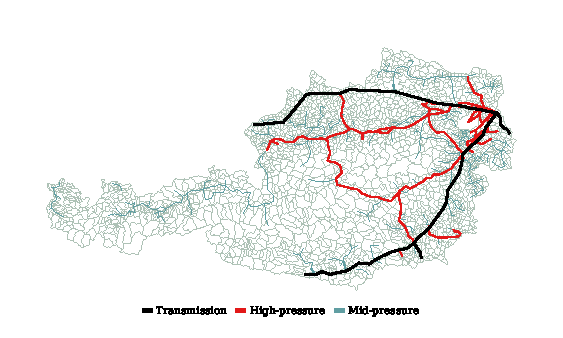
\includegraphics[width=1\linewidth]{figures/results/gas_grid_2030_all_scenarios.pdf}
	\caption{Austrian gas grid in 2030 at the transmission (blue), high-pressure (red) and mid-pressure (green) pressure levels in all four scenarios.}
	\label{fig_grid_2030}
\end{figure}

The main reason for the reduction is the use of redundancies and duplicate structures in the grid as a result of declining gas demand. Table \ref{tab_compare_initial_2030} shows the reduction in the grid length at the high-pressure and mid-pressure levels in the four scenarios. 

\begin{table}[h]
	\centering
	\setlength{\extrarowheight}{.5em}
	\resizebox{0.9\textwidth}{!}{
		\begin{tabular}{lccccc}
			\toprule
			& 2025 & \multicolumn{4}{c}{2030}\\\cmidrule(lr){2-2}\cmidrule(lr){3-6}
			Pressure level & Initial grid & Elec & GG & DGG & GM\\\cmidrule(lr){1-2}\cmidrule(lr){3-6}
			\multirow{2}{*}{High-pressure} & \multirow{2}{*}{\SI{1449}{km}} & \SI{-172}{km}  & \SI{-142}{km} & \SI{-142}{km}  & \SI{-131}{km}\\
			&  & (\SI{-11.9}{\%}) & (\SI{-9.8}{\%}) & (\SI{-9.8}{\%}) & (\SI{-9.0}{\%})\\\hdashline
			\multirow{2}{*}{Mid-pressure} & \multirow{2}{*}{\SI{3218}{km}} & \SI{-283}{km}  & \SI{-200}{km} & \SI{-186}{km}  & \SI{-208}{km}\\
			& & (\SI{-8.8}{\%}) & (\SI{-6.2}{\%}) & (\SI{-5.8}{\%}) & (\SI{-6.5}{\%})\\
			\bottomrule
	\end{tabular}}
	\caption{Absolute and relative reduction in the length of the gas grid at the high-pressure and mid-pressure levels by 2030 compared to the initial grid in 2025. Abbreviations: Electrification (Elec), Green Gases (GG), Decentralized Green Gases (DGG), Green Methane (GM).}
	\label{tab_compare_initial_2030}
\end{table}

The reduction in the grid length at the high-pressure level varies between \SI{-131}{km} and \SI{-172}{km} in the GM and Elec scenarios respectively. The reduction in the grid length at the mid-pressure level varies between \SI{-186}{km} and \SI{-283}{km} in the DGG and Elec scenarios respectively. Removing redundant gas pipelines reduces the operating costs of the grid.\footnote{In reality, these gas pipelines, especially at the transmission and high-pressure levels, can form the core of a hydrogen network. For further details, see for example, the plans for the Austrian hydrogen grid by 2030 published by the Austrian gas network operator \cite{aggm_agid}.} The operating costs of the gas grid, which are mainly fixed pipeline costs, decrease compared to the initial grid in 2025 and are around \SI{110}{MEUR} in all four scenarios in 2030. Note that energy costs for the compressor are not included. By 2030, virtually no gas pipelines are decommissioned due to ageing or because the pipeline is no longer used to transport gas. The assumed young grid age also leads to very low replacement investments into the gas grid. In total, those investments vary by 2030 between \SI{15}{MEUR} and \SI{18}{MEUR} in the Elec and GM scenarios respectively. Note that in the model here, replacement investment is necessary when a pipeline reaches its technical lifetime of \SI{75}{years}. At this point, the model decides whether to invest in replacing the pipeline or to decommission it due to its age. 

\subsection{Austrian gas grid in 2040}\label{res_grid2040}
The Austrian gas grid in 2040 differs significantly between the four scenarios. Four different gas grids emerge, which are mainly determined by the assumptions of the underlying scenarios. Figures \ref{fig_grid_2040_small} and \ref{fig_grid_2040_large} show the smallest and largest gas grids in terms of grid length. 

\begin{figure}[h]
	\centering
	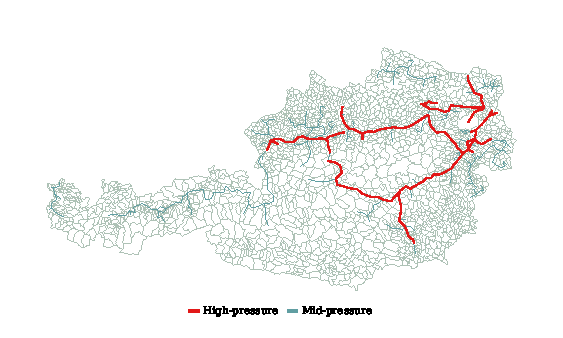
\includegraphics[width=1\linewidth]{figures/results/gas_grid_2040_elec_cleaned.pdf}
	\caption{Austria's smallest gas network by 2040 in the scenario Electrification (Elec). Colours: transmission (blue), high-pressure (red) and mid-pressure (green).}
	\label{fig_grid_2040_small}
\end{figure}

The smallest grid is in the Elec scenario and the largest in the GM scenario. The gas grids of the remaining two scenarios GG and DGG are shown in \ref{app_results_2040_extension}. They lie between the two extreme grids in terms of size. Table \ref{tab_compare_initial_2040} quantifies the size of the gas grids in 2040 in all the four scenarios by comparing the absolute length of the grids as well as the absolute and relative reduction of grid lengths compared to the initial grid in 2025.  In absolute numbers, the reduction of grid length at the mid-pressure level is more significant than at the high-pressure level. In particular, the reduction in the grid length at the mid-pressure level is equally greatest in the two scenarios Elec and GG the greatest with \SI{-1316}{km} and  \SI{-40.9}{\%} compared to the initial grid in 2025. The smallest reduction in length at the mid-pressure level among the four scenarios is with \SI{-811}{km} (\SI{-40.9}{\%}) compared to the initial grid in 2025) in the DGG scenario. 

\begin{figure}[h]
	\centering
	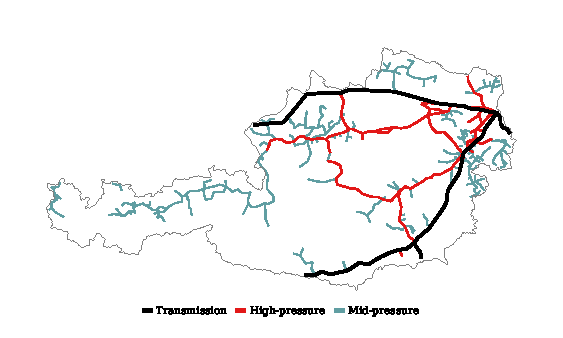
\includegraphics[width=1\linewidth]{figures/results/gas_grid_2040_gm.pdf}
	\caption{Austria's largest gas network by 2040 in the scenario Green Methane (GM). Colours: transmission (blue), high-pressure (red) and mid-pressure (green).}
	\label{fig_grid_2040_large}
\end{figure}

The main reason here for the relatively small reduction in the mid-pressure grid length is the significant decentralized production and injection of renewable gas. 

\begin{table}[h!]
	\centering
	\setlength{\extrarowheight}{.5em}
	\resizebox{1\textwidth}{!}{
		\begin{tabular}{llrrrr}
			\toprule
			& & \multicolumn{4}{c}{2040}\\\cmidrule(lr){3-6}
			Pressure level & Indicator & \multicolumn{1}{c}{Elec} & \multicolumn{1}{c}{GG} & \multicolumn{1}{c}{DGG} & \multicolumn{1}{c}{GM}\\\cmidrule(lr){1-2}\cmidrule(lr){3-6}
			\multirow{3}{*}{High-pressure} & Abs. grid length in 2040& \SI{964}{km}  & \SI{965}{km} & \SI{974}{km}  & \SI{1105}{km}\\
			 & Abs. reduction to 2025 & \SI{-485}{km}  & \SI{-484}{km} & \SI{-475}{km}  & \SI{-344}{km}\\
			 & Rel. reduction to 2025 & \SI{-33.5}{\%}& \SI{-33.4}{\%}& \SI{-32.8}{\%}&\SI{-23.7}{\%}\\\hdashline
 			\multirow{3}{*}{Mid-pressure} & Abs. grid length in 2040& \SI{1902}{km}  & \SI{1902}{km} & \SI{2407}{km}  & \SI{2331}{km}\\
			 & Abs. reduction to 2025 & \SI{-1316}{km}  & \SI{-1316}{km} & \SI{-811}{km}  & \SI{-887}{km}\\
			 & Rel. reduction to 2025 & \SI{-40.9}{\%}& \SI{-40.9}{\%}& \SI{-25.2}{\%}&\SI{-27.6}{\%}\\
			\bottomrule
	\end{tabular}}
	\caption{Absolute length of the grids 2040 in the four scenarios as well as the absolute and relative reduction of grid lengths compared to the initial grid in 2025 at the high-pressure and mid-pressure levels. Abbreviations: Electrification (Elec), Green Gases (GG), Decentralized Green Gases (DGG), Green Methane (GM).}
	\label{tab_compare_initial_2040}
\end{table}

The injection leads to an increased use of mid-pressure pipelines. Figure \ref{fig_reduction_waterfall} shows the grid length in the two extreme scenarios Elec (top) and GM (bottom) at high-pressure (left) and mid-pressure (right) levels. It highlights the reduction in grid length by 2030 and 2040. The grid length in 2025 is shown on the far left and in 2040 on the far right. 

\begin{figure}[h]
	\begin{subfigure}[c]{0.5\textwidth}
		\centering
		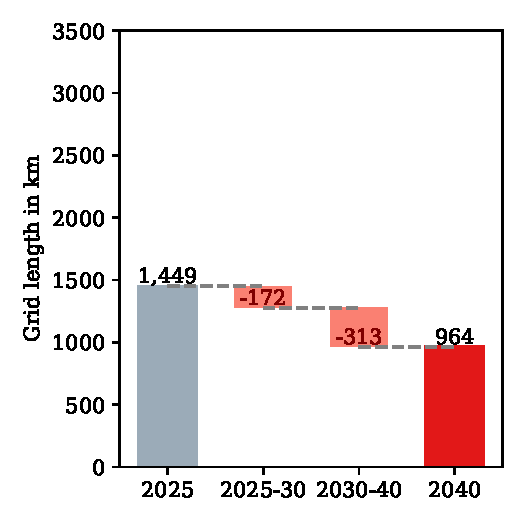
\includegraphics[width=1\linewidth]{figures/results/waterfall/waterfall_elec_high.pdf}
		\vspace{-0.6cm}
		\subcaption{Elec | High-pressure}
		\label{Fig:a}
	\end{subfigure}
	\begin{subfigure}[c]{0.5\textwidth}
		\centering
		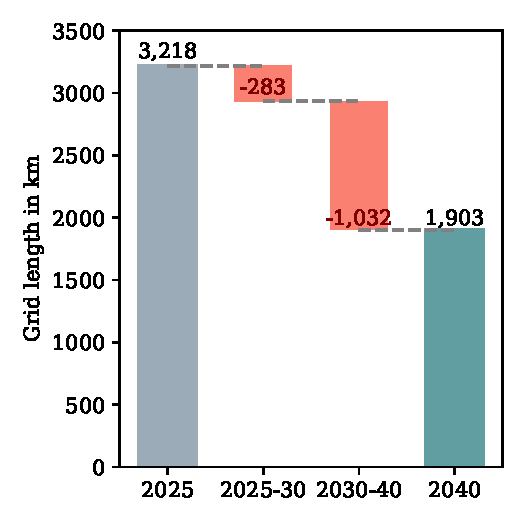
\includegraphics[width=1\linewidth]{figures/results/waterfall/waterfall_elec_mid.pdf}
		\vspace{-0.6cm}
		\subcaption{Elec  | Mid-pressure}
		\label{Fig:b}
	\end{subfigure}
	\newline
	\newline
	\newline
	\begin{subfigure}[c]{0.5\textwidth}
		\centering
		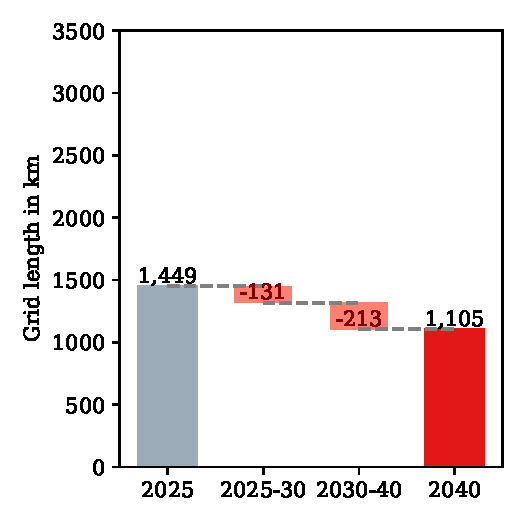
\includegraphics[width=1\linewidth]{figures/results/waterfall/waterfall_gm_high.pdf}
		\vspace{-0.6cm}
		\subcaption{GM | High-pressure}
		\label{Fig:c}
	\end{subfigure}
	\begin{subfigure}[c]{0.5\textwidth}
		\centering
		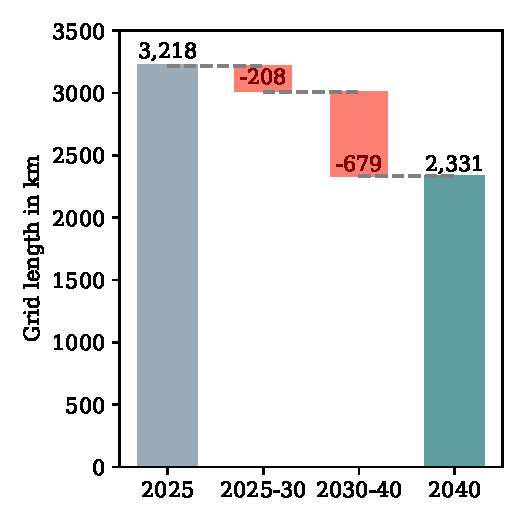
\includegraphics[width=1\linewidth]{figures/results/waterfall/waterfall_gm_mid.pdf}
		\vspace{-0.6cm}
		\subcaption{GM | Mid-pressure}
		\label{Fig:d}
	\end{subfigure}
	\caption{Comparison of the Austrian gas grid in 2025 and 2040 in the scenarios extreme scenarios Electrification (Elec) and Green Methane (GM) at high-pressure and mid-pressure levels. In the Elec and GM scenarios, the smallest and the largest gas grids are obtained in terms of the size of the grids.}
	\label{fig_reduction_waterfall}
\end{figure}

The operating costs of the gas grid decrease compared to 2025. They vary between \SI{87.5}{MEUR} and \SI{93.0}{MEUR} in the Elec and GM scenarios respectively. \SI{50.0}{MEUR} (the same in all four scenarios) are accounted for the transmission level. The remaining costs are accounted for the high-pressure and mid-pressure level. Figure \ref{fig_grid_repl_inv} shows the total replacement investments in the gas grid in the four scenarios. It includes the replacement investments in 2030 mentioned in Section \ref{res_grid2030} above. The lowest total replacement investments are in the scenarios GG and Elec with \SI{143.0}{MEUR} and \SI{146.0}{MEUR} respectively. The highest replacement investments are in the GM scenario with \SI{185.0}{MEUR}. 

\begin{figure}[h]
	\centering
	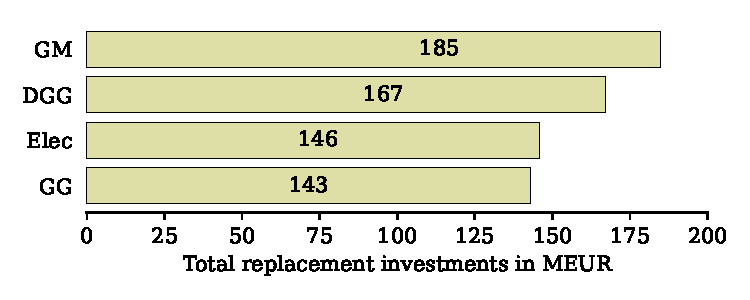
\includegraphics[width=0.8\linewidth]{figures/results/total_replacement_inv/replace_inv_2040.pdf}
	\caption{Total replacement investments in the Austrian gas grid until 2040 in the four scenarios.}
	\label{fig_grid_repl_inv}
\end{figure}

\subsection{Grid charges for customers in 2040}\label{res_grid_charges}
This section presents an analysis of the cost-effectiveness of the gas grid in four different scenarios. The average grid costs are calculated by dividing the total annual grid costs by the gas demand supplied by the grid, and these figures are provided. These average grid costs serve as a basis for estimating grid charges for customers in 2040. It should be noted that determining grid charges based on minimizing system costs is challenging due to regulatory considerations. Nevertheless, regulatory mechanisms often rely on approaches that aim to minimize system costs. Therefore, it is important to consider and interpret the following results from this perspective. In particular, the different grid costs provide a different perspective on comparing the four scenarios.\vspace{0.3cm}

Figure \ref{fig_grid_charges} shows the (average) grid costs in 2040 in the four different scenarios. Note that the horizontal axis is the gas demand supplied by the grid in TWh. The Elec scenario is therefore on the far left, as it has the lowest gas demand of the four scenarios. At the same time, the GM scenario, which has the highest gas demand among the scenarios, is on the far right. 

\begin{figure}[h]
	\centering
	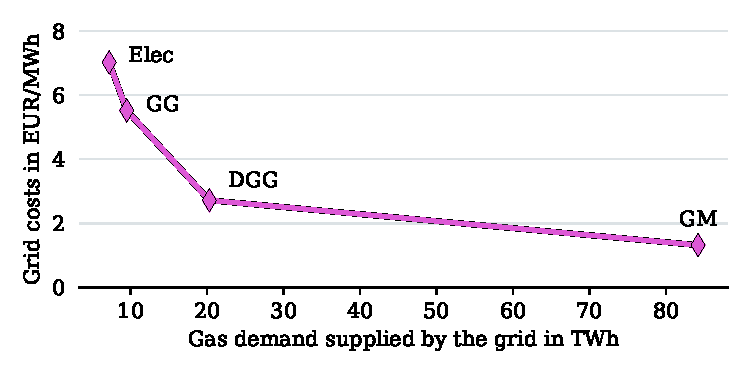
\includegraphics[width=1\linewidth]{figures/results/grid_charges/grid_charges.pdf}
	\caption{Total replacement investments in the Austrian gas grid until 2040 in the four scenarios.}
	\label{fig_grid_charges}
\end{figure}

It is shown that the grid costs are the highest in the Elec scenario with \SI{7.0}{EUR \per MWh} and the lowest in the GM scenario with \SI{1.3}{EUR \per MWh}. The grid costs and its components of operating costs at the different pressure levels and gas demand supplied are summarized in Table \ref{tab_components_grid_costs}.

\begin{table}[h!]
	\centering
	\setlength{\extrarowheight}{.5em}
	\resizebox{0.85\textwidth}{!}{
		\begin{tabular}{lrrrr}
			\toprule
			& \multicolumn{4}{c}{2040}\\\cmidrule(lr){2-5}
			Components for calculating grid costs & Elec & GG & DGG & GM\\\hline
			Transmission operating costs in MEUR & 0 & 0 &0  & \SI{50}{}\\
			Distribution operating costs in MEUR & \SI{37.5}{} & \SI{39.3}{} & \SI{40.2}{} & \SI{43.0}{}\\
			Capital expenditure in MEUR & \SI{13.0}{} & \SI{13.1}{} & \SI{15.0}{} & \SI{18.3}{}\\
			Gas demand supplied in TWh & \SI{7.2}{} & \SI{9.5}{} & \SI{20.3}{} & \SI{84.2}{}\\\hline
			Grid costs in EUR/MWh & \SI{7.0}{} & \SI{5.5}{} & \SI{2.7}{} & \SI{1.3}{}\\
			\bottomrule
	\end{tabular}}
	\caption{Average grid costs and their components of operating costs and capital expenditure. The distribution operating costs encompass the high-pressure and mid-pressure levels. Separation between the transmission and distribution grids result in no transmission operating costs for the customers.}
	\label{tab_components_grid_costs}
\end{table}

Note that the three scenarios Elec, GG and DGG assume a separation between the transmission and distribution grids (i.e., high and medium pressure levels). Therefore, the transmission operating costs for customers in these scenarios are zero. Consequently, it is assumed that customers requesting gas transport through Austria at the transmission level bear these costs. \textcolor{red}{Hier gehts morgen weiter.} 

\begin{figure}[h]
	\centering
	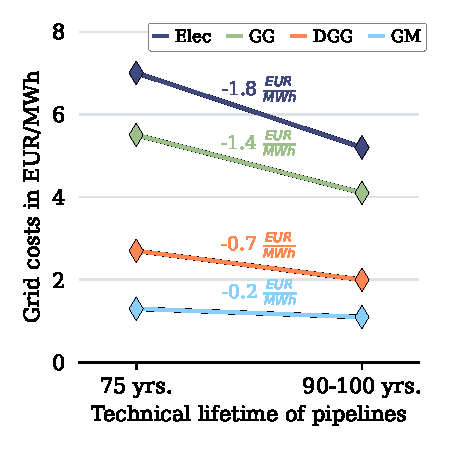
\includegraphics[width=0.5\linewidth]{figures/results/grid_charges_development/cleaned_grid_charges.pdf}
	\caption{}
	\label{fig_grid_charges_no_capex}
\end{figure}

Overestimate the replacement investment costs. 

\section{Synthesis}\label{synthesis}
% In a first sub-section, you should refer to your research questions in Chapter 1 again and focus on whether / how they have been answered

% Secondly, explain whether upscaling and transferability of the results is possible under varying framework conditions / circumstances / boundaries (spatially, temporally, sociologically, etc.)

% Thirdly, explain the strengths and limitations of the methodology used and the lessons learned

% gemeinsame Nutzung von Biogasanlagen

\newpage
\section{Conclusions}\label{conclusions}
was es wert diese analyse durchzuführen: nicht nur mengen, sondern auch einspeisung und deren verortung.


die zukunft von erdgasnetzen bleibt eine der spannendsten fragen die sich durch die umsetzung der dekarbonisierung ergibt. 

unbestritten, wird es zu einer verkleinerung der erdgasnetze kommen.

auf der fernleitungsebene sehr eindeutig, dass eine umwidmung zu wasserstoff möglich ist, weil kapazitäten vorhanden sind. parallelstränge erlauben es

auf der verteilnetzebene nicht mehr so eindeutig. 

doppelstrukturen herauslösen weil netz oft redundanzen hat.

setzt man auf biomethane große netze weiter gebraucht.

dabei kommt es weniger auf die absoluten mengen an, sondern die verteilte einspeisung ist eher eine ja/nein entscheidung

teurere netze, selbst im elektrifizierung noch ein großes netz 

schaffen regional/lokal biomethan, genau abgestimmt wo weiterhin verbrauch bleibt

zukünftige arbeiten, diese regionalen cluster zu identifizieren
weitere technische details berücksichtigen, wie die druckentwicklung in schwächer ausgelasteten netzen, energie die gebraucht wird um druckhertzstellen, etc.

\newpage
\section*{Declaration of interests}
None.
\section*{Declaration of Competing Interest}
The authors report no declarations of interest.
\section*{Acknowledgments}


\bibliography{mybibfile}
\appendix
\setcounter{table}{0}
\setcounter{figure}{0}

\section{Detaillierte Gasnetz im Szenario A und B 2040}\label{app_results_2040_extension}
%
%\begin{sidewaystable}
%	\centering
%	\setlength{\extrarowheight}{.5em}
%	\resizebox{1\textwidth}{!}{
%		\begin{tabular}{cclll}
%			\toprule
%			\multicolumn{2}{c}{Equation} & \multicolumn{3}{c}{Qualitative/high-level explanation of the mathematical formulation}\\\cmidrule(lr){1-2}\cmidrule(lr){3-5}
%			Number & Dimension & Type & Keyword & Description\\\hline
%			\ref{objective} & 1 & Economic & Objective &  Minimize gas network operator's total costs\\
%			\ref{eq:capex} & 1 & Economic  & Capex &  Capital cost of the gas pipelines\\
%			\ref{eq:opex} & 1 & Economic & Opex & Fixed operating costs of gas pipelines\\
%			\ref{eq:total_book_value} & ($p \times l \times y$) & Economic & Book values & Book value per gas pipeline, network level and year\\
%			\ref{eq:revenues} & ($n \times l \times y \times m$) & Economic & Revenues & Revenues for supplying gas demand through network charge\\
%			\ref{bound1}, \ref{bound2} & ($p \times l \times y$) & Technical & Gas transport & Restriction of the gas transport per gas pipeline, network level and year\\
%			\ref{eq:balance} & ($n \times l \times y \times m$) & Technical & Gas balance & Gas balance constraint per node, network level, year and month\\
%			\ref{eq:demand} &  ($n \times l \times y \times m$) & Technical & Gas demand & Total gas demand as sum of local demand and delivered gas\\
% 			\ref{eq:source} &  ($n \times l \times y \times m$) & Technical & Gas source & Total gas source as sum of local production and gas delivered\\
%			\bottomrule
%	\end{tabular}}
%	\caption{\added{Overview of the model's mathematical formulation. Abbreviations: Gas pipeline (p), Network level (l), Node (n), Year (y), Month (m)}}
%	\label{tab:brief}
%\end{sidewaystable}
%
%\section{Current natural gas demands in Vorarlberg, Austria}\label{app_demand}
%Figure \ref{fig:comp} shows current natural gas demands in Vorarlberg, Austria. The left subfigure shows natural gas demands in Vorarlberg, Austria, in 2018 and 2025. Open data and information from the internal database \cite{EEG} are used to split 2018's values into industry and (building) heating. The values are available at the provincial level (i.e., Vorarlberg, Austria). The 2025's values are calculated bottom-up. That means that we use data on natural gas demands at the community level (between 2018 and 2025). Note that the difference between 2018's and 2025's gas demands reflects the lack of gas demand data at the community level only. 
%
%\begin{figure}[h]
%	\centering
%	\includegraphics[width=0.75\linewidth]{figures/Comparison_of_the_demand.eps}
%	\caption{Overview of gas demands in 2018 and 2025 (left) and share of natural gas in total energy demand (right). Data: open data available; Avg.: shares calculated based on the average gas demand per capita in Vorarlberg, Austria; All: Data and Avg. combined.}
%	\label{fig:comp}
%\end{figure}
%
%The right subfigure indicates the approach to calculating gas demands if no open data are available. It shows the share of natural gas demands in energy demand at the community level. The first item (Data) shows the distribution for those communities where data are available. The second item (Avg.) shows the distribution of gas demand shares using the average value of gas demand per capita in Vorarlberg, Austria. This calculation process based on the average gas demand is used for communities where no data are available. The third item (All) shows the distribution of gas demand shares for all communities.
%
%
%
%\section{Assumptions regarding lumpiness of gas pipelines}\label{app:lum}
%Similar to \cite{von2006reform}, we assume a simplified relationship between the diameter of gas pipelines and their capacities. Accordingly, we assume that the capacity of high- and mid-pressure gas pipelines increases by 2.5 times the power of the diameter. Table \ref{tab:lum} summarizes the set of potential diameters and the corresponding calculated capacity. 
%
%\definecolor{Gray}{gray}{0.95}
%\begin{table}[h]
%	\centering
%	\scalebox{1}{
%			\renewcommand{\arraystretch}{1.4}
%			\begin{tabular}{c|c}
%					Diameter in meters & Pipeline capacity in MW\\\hline
%					0.1 & 0.82\\
%					0.2 & 4.62\\
%					0.3 & 12.72\\
%					0.4 & 26.11\\
%					0.5 & 45.62\\
%					0.6 & 71.96\\
%					0.7 & 105.8\\
%					0.8 & 147.73\\
%					0.9 & 198.31\\
%					1.0 & 258.07\\
%					1.1 & 327.51\\
%					1.15 & 366.0\\
%					1.2 & 407.09\\
%					1.3 & 497.27\\
%			\end{tabular}}
%	\caption{Set of diameters of gas pipelines and assumed pipeline capacity.}
%	\label{tab:lum}
%\end{table}
\end{document}